\documentclass[9pt,twoside]{pnas-new}

\articletype{Social Sciences}
\templatetype{pnasmathematics}

\usepackage[section]{placeins}
\usepackage{caption}
\usepackage{booktabs}
\usepackage{graphicx}
\renewcommand{\topfraction}{0.85}
\renewcommand{\bottomfraction}{0.85}
\renewcommand{\textfraction}{0.10}
\renewcommand{\floatpagefraction}{0.80}
\setcounter{topnumber}{3}
\setcounter{bottomnumber}{2}
\setcounter{totalnumber}{5}
\setlength{\floatsep}{5pt plus 2pt minus 2pt}
\setlength{\textfloatsep}{6pt plus 2pt minus 2pt}
\setlength{\intextsep}{5pt plus 2pt minus 2pt}
\setlength{\dbltextfloatsep}{6pt plus 2pt minus 2pt}
\setlength{\abovecaptionskip}{3pt}
\setlength{\belowcaptionskip}{0pt}
\captionsetup{skip=3pt}

\begin{document}

\title{Direction Without Degree: Party Control, Majority Size, and Medicaid Restriction in a State Panel, 2015--2026}

\author[a,1]{Ben Floman}
\affil[a]{Quantitative Social Science, Dartmouth College, Hanover, NH 03755}
\leadauthor{Floman}

\significancestatement{Whether a state runs its safety-net programs generously is usually explained by which party controls the legislature. A natural next question is whether the \emph{size} of that majority matters too---whether a 70-percent majority governs differently from a bare one. For Medicaid restriction the answer is that it does not: partisan influence here operates as a switch, not a dial. Which party controls the chamber predicts whether a state attaches restrictive Medicaid waivers---Democratic-controlled expansion states never do---but among the states that use the tool, larger majorities do not use it more. The apparent ``more majority, more restriction'' gradient predicts not a single restriction in a held-out state and disappears when one state is removed. For this policy, holding the majority is what matters; the data detect no effect of its size. The result also carries a methodological warning: in panels where an institutional regressor barely moves within units, a standard fixed-effects model returns a ``size'' coefficient that looks continuous but is a between-state contrast in disguise, and only out-of-sample validation reveals the difference.}

\authorcontributions{B.F.\ designed the study, assembled the data, performed the analysis, and wrote the paper.}
\authordeclaration{The author declares no competing interests.}
\correspondingauthor{\textsuperscript{1}E-mail: ben.floman.28@dartmouth.edu}

\begin{abstract}
Accounts of state policy usually treat legislative control as binary---which party holds the majority. Veto-player theory suggests the \emph{size} of that majority should matter too, and continuously: larger majorities, more unilateral capacity. This paper tests that prediction against an alternative---that partisan influence operates as a threshold rather than a gradient---using a monthly panel of 49 states from 2015 through 2026 and two outcomes: the breadth of Medicaid enrollment relative to the low-income population, and the use of restrictive Section 1115 waivers (work requirements, premiums, enrollment caps). For restriction the threshold account wins: the behavior is a switch, not a dial. Restrictive waivers are a partisan instrument that no Democratic-controlled expansion state imposes, but among the states that use the tool, magnitude does not modulate use. The one place a continuous effect appears---a positive seat-margin coefficient on enrollment---is the apparent dial, and it dissolves under scrutiny: it is identified almost entirely off the Republican end of the range, cannot be separated from the binary control indicator (the two correlate at $r=0.86$ within expansion states), and the within-party slopes are not distinguishable. A classifier trained to predict restriction from seat margin achieves an in-sample F1 of 0.72 but a leave-one-state-out F1 of 0.00; an $L_1$-penalized model discards margin and keeps only party control; the gradient reverses when a single state is removed; and two placebo samples return null. The result is consistent with a threshold and inconsistent with any detectable continuous gradient: for Medicaid restriction, holding the majority is what matters, not its size.
\end{abstract}

\dates{This manuscript was compiled on \today}
\doi{\url{https://www.pnas.org/cgi/doi/10.1073/pnas.XXXXXXXXXX}}

\maketitle
\thispagestyle{firststyle}
\ifthenelse{\boolean{shortarticle}}{\ifthenelse{\boolean{singlecolumn}}{\abscontentformatted}{\abscontent}}{}

\Firstpage

\dropcap{T}he standard model of partisan politics treats legislative control as binary: a party either holds a majority or it does not. That framing arguably misses something. A party with 51 percent of lower-chamber seats and one with 70 percent both have a majority, but they operate under different coalition dynamics---a narrow majority can be paralyzed by a handful of defectors, while a dominant one absorbs them. Majority \emph{size} may carry information that the binary indicator of direction cannot. This paper tests that idea in the setting of Medicaid implementation and finds the opposite: partisan influence on Medicaid restriction operates as a switch, not a dial. Which party controls the chamber governs whether a state restricts; how large the majority is does not.

Medicaid is a useful setting because implementation runs in two directions. The Affordable Care Act let states expand eligibility in 2014; afterward a state can ease enrollment through outreach and lenient renewals, or tighten it through work requirements, premiums, and enrollment caps. Rocco et al.\ \cite{rocco2020} establish that partisan \emph{control} is the dominant predictor of expansion adoption. The narrower question here is whether, conditional on direction, the \emph{size} of a majority is associated with how a state implements the program afterward.

The theoretical motivation is Tsebelis's veto-player theory \cite{tsebelis2002}: larger majorities have fewer effective internal veto players, enabling more unilateral action---continuously in seat share, not merely at a 50-percent threshold. This predicts a \emph{dial}: restriction should rise with the size of the controlling majority. The competing hypothesis is a \emph{switch}: applying for or declining a restrictive waiver is a discrete act that turns on whether a party controls the chamber, and once it does, additional seats add little marginal capacity for that particular action. The paper adjudicates between these forms and finds for the switch---and, along the way, shows why a standard two-way fixed-effects panel can appear to support the dial when it does not, because the regressor barely moves within states and a coefficient that looks like a ``size effect'' is in fact a between-state contrast that does not generalize.

\section*{Theoretical Background}

Tsebelis \cite{tsebelis2002} shows that the scope for policy change shrinks as the number of effective veto players grows, and within a chamber majority size sets that number. Taken at face value this implies a dial: a larger majority faces fewer internal veto points and can act more aggressively, so restriction should scale with seat share. But the prediction depends on the policy being the kind of thing extra seats help with. Medicaid restriction may not be. Applying for a Section 1115 waiver---or declining to---is a discrete executive-and-legislative action: it requires a party to control the agenda and the relevant committees, but once it does, a bare majority and a supermajority can file the same application. Nor does a larger majority obviously buy more aggressive restriction: how far a waiver can go---whether it can layer work requirements, premiums, and enrollment caps at once---is bounded by federal approval and state administrative capacity rather than by seat count, so the marginal seat adds little. On this account the binding constraint is \emph{holding} the majority, not its size, and the relationship is a switch. The two accounts make different empirical predictions---a continuous margin gradient under the dial, a flat within-party relationship with a discontinuity at control under the switch---and the rest of the paper tests between them.

A second asymmetry sharpens the switch reading. Restriction is a one-sided instrument: a Republican majority can pursue work requirements, premiums, and enrollment caps, as in Idaho and Utah \cite{jarlenski2020}, while the platform of the expanding party forecloses them, so Democratic-controlled states sit at zero by construction. Stimson et al.\ \cite{stimson1995} supply a complementary median-shift channel; Gilens and Page \cite{gilenspage2014} caution that elite preferences can override the median voter, and the citizen-ideology control is meant to separate caucus-internal capacity from statewide opinion, if imperfectly. The paper extends the binary baseline of Rocco et al.\ \cite{rocco2020}---control predicts adoption---from the discrete question of whether a state restricts to the continuous question of whether, among those that do, larger majorities restrict more.

\section*{Data}

\textbf{Sources.} The analysis combines four public sources. Monthly Medicaid and CHIP enrollment comes from the Kaiser Family Foundation's (KFF) State Health Facts, January 2014--January 2026. The poverty denominator comes from U.S.\ Census Bureau ACS 1-year estimates, table C17002, 2014--2023. Lower- and upper-chamber partisan composition comes from the NCSL Partisan Composition Database. Statewide opinion is a citizen-ideology measure in the Berry et al.\ tradition \cite{berry1998}. Restrictive-waiver status is coded from the public record of approved Section 1115 demonstrations.

\textbf{Outcomes.} The first outcome is total Medicaid and CHIP enrollment divided by the state population below 138 percent of the federal poverty line, times 100. I call it the enrollment ratio; it is a coverage-breadth index, not a literal take-up rate. The numerator includes CHIP children, the elderly and disabled, and pregnant women, many outside the sub-138\% denominator, so the ratio exceeds 100 percent for most states (mean 119.5). Because the numerator is broad, the within-state movement the model identifies is not cleanly the legislative channel---state-specific shocks such as unemployment move enrollment, and year effects remove only their national component. I therefore treat the enrollment regression as corroboration, not as a clean estimate of a legislative effect. The second outcome---the one the design can actually resolve---is a binary indicator for whether an expansion state-year carries an active restrictive waiver (work requirements, premiums, or enrollment caps).

\textbf{Key regressor.} \emph{Dem.\ Seat Margin} is the Democratic share of lower-chamber seats minus 0.5; positive values indicate a Democratic majority. A binary \emph{Dem.\ Control} indicator captures direction.

\textbf{Limitations and missingness.} The 2020 ACS 1-year file was suspended, so 2020 uses the ACS 5-year estimate; ACS ends in 2023, so 2024--2026 denominators are forward-filled (a static-denominator check confirms this does not drive results). Most consequentially, NCSL composition is observed at only five snapshots, so the key regressor changes at most five times per state---a binding constraint on identification developed below. Non-numeric enrollment cells in the raw KFF file are dropped. Table~\ref{tab:desc} reports summary statistics.

\section*{Methods}

\textbf{Panel specification.} The primary model is a two-way fixed-effects regression estimated by OLS with state-clustered standard errors:
\[
\mathrm{Ratio}_{it}=\alpha+\beta_1\mathrm{Margin}_{it}+\beta_2\mathrm{DemCtrl}_{it}+\beta_3\mathrm{PostExp}_{it}+\beta_4\mathrm{Mood}_{it}+\gamma_i+\delta_t+\varepsilon_{it},
\]
where $i$ indexes states and $t$ months. State fixed effects $\gamma_i$ absorb time-invariant cross-state differences; year fixed effects $\delta_t$ absorb common annual shocks. The COVID-19 continuous-enrollment period (March 2020--April 2023) is flagged with a binary indicator and excluded in robustness checks. Errors are clustered by state. The panel drops 2014, Nebraska (unicameral), and DC, leaving 4{,}118 state-months across 49 states.

\textbf{Identification, stated plainly.} This is an inferential, not a clean causal, design, and its central limitation is not subtle. With state fixed effects, $\beta_1$ is identified from within-state movement in seat margin, but margin changes at most five times per state and only one partisan control flip (Minnesota, 2019) occurs in the entire panel. The reported $N$ of 4{,}118 reflects the monthly outcome, not the variation in the regressor; precision should be read accordingly. The remainder of the analysis is built around this constraint rather than against it: I ask what can be learned about \emph{direction}, which the data do contain, and I show why the apparent evidence for \emph{size} does not hold up.

\textbf{Restriction as a classification problem.} Because the substantive claim about size is sharpest for restrictive waivers, and because the waiver outcome is binary, I treat it as a supervised classification target. I fit an interpretable depth-3 decision tree predicting restriction from \{seat margin, control, governor party\}, and---critically---evaluate it under \emph{leave-one-state-out} cross-validation. Grouping the folds by state, rather than by random row, is the correct evaluation for serially correlated panel data: a naive split would train on a state's 2018 to predict its 2019 and report inflated performance. Leave-one-state-out asks the question that matters for a \emph{generalizable} size effect---can the model predict a held-out state's restriction from the other states' margins? I complement the tree with an $L_1$-penalized (Lasso) logistic regression, which both performs variable selection between direction and size and converges under the perfect class separation that prevents an ordinary logit from fitting.

\textbf{Placebos.} Placebo A restricts to non-expansion state-months (no expansion population to restrict); Placebo B restricts to pre-expansion months for late expanders. Both reuse the two-way FE specification.

\begin{table}[htbp]
\centering
\caption{Descriptive statistics for the analysis sample}
\label{tab:desc}
\small
\begin{tabular}{lrrrrr}
\toprule
Variable & $N$ & Mean & SD & Min & Max\\
\midrule
Enrollment ratio (\% of $<$138\% FPL) & 4{,}118 & 119.5 & 39.2 & 58.6 & 230.4\\
Dem.\ Seat Margin & 4{,}118 & $-0.08$ & 0.21 & $-0.42$ & 0.42\\
Dem.\ Control (0/1) & 4{,}118 & 0.31 & 0.46 & 0 & 1\\
Post-Expansion (0/1) & 4{,}118 & 0.60 & 0.49 & 0 & 1\\
Citizen ideology (mood) & 4{,}118 & 0.45 & 0.11 & 0.22 & 0.66\\
COVID Period (0/1) & 4{,}118 & 0.24 & 0.43 & 0 & 1\\
\bottomrule
\end{tabular}
\addtabletext{Panel covers January 2015--January 2026; Nebraska and DC excluded. The enrollment ratio exceeds 100\% by construction (see Data).}
\end{table}

\section*{Results}

\textbf{The switch: control governs restriction.} The behavior the theory is really about is whether a state restricts, and there party control is decisive (Fig.~\ref{fig:quartile}). No Democratic-controlled expansion state has ever imposed a restrictive waiver; restriction appears only under Republican control. This separation is partly definitional---restriction is a Republican instrument---but it establishes the switch: crossing from Democratic to Republican control turns the behavior on, with Democratic states pinned at zero by platform. The open question is what happens \emph{past} that threshold---among the states that use the tool, does a larger majority use it more (the dial), or does holding control exhaust the relationship (the switch)?

\begin{SCfigure*}[\sidecaptionrelwidth][htbp]
\centering
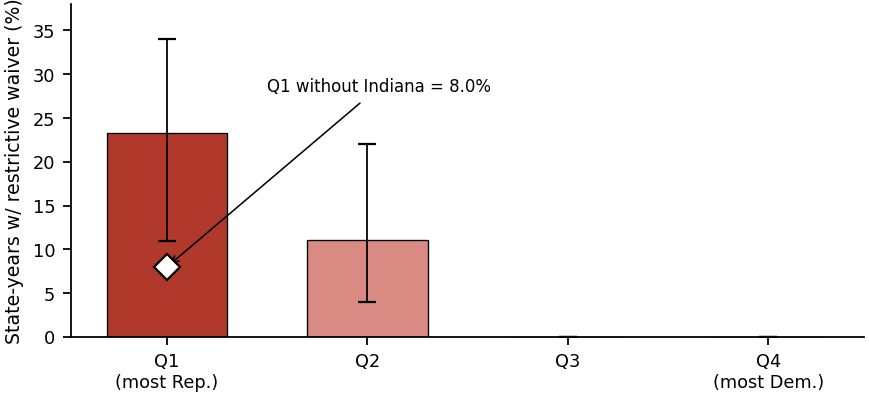
\includegraphics[width=0.60\linewidth]{fig_waiver_quartile.png}
\caption{Restrictive-waiver prevalence by Democratic seat-margin quartile, expansion states; whiskers are 95\% CIs. The zero floor in the Democratic quartiles reflects the instrument's partisan nature. The within-Republican Q1$>$Q2 gap reverses when Indiana is removed (marker), showing the gradient rests on one state.}
\label{fig:quartile}
\end{SCfigure*}

\textbf{The apparent dial.} One result looks like a dial. In the full sample the continuous seat margin is a positive, significant predictor of the enrollment ratio---80.9 points per unit of share (SE $=31.5$, $p=0.010$; 86.9 excluding COVID)---while the binary control indicator is small and insignificant (Table~\ref{tab:panel}). Taken at face value this is the dial: enrollment rising smoothly with Democratic seat share. The rest of this section shows it is an artifact.

\begin{table}[htbp]
\centering
\caption{Two-way fixed-effects estimates and placebo samples}
\label{tab:panel}
\small
\begin{tabular}{lrrrr}
\toprule
& \multicolumn{2}{c}{Main} & \multicolumn{2}{c}{Placebo}\\
\cmidrule(lr){2-3}\cmidrule(lr){4-5}
& (1) Full & (2) Excl.\ COVID & (A) Non-exp. & (B) Pre-exp.\\
\midrule
Dem.\ Seat Margin & $80.85^{**}$ & $86.85^{**}$ & 24.71 & 3.82\\
 & (31.53) & (35.79) & (30.23) & (33.33)\\
Dem.\ Control & $-1.90$ & $-5.49$ & --- & ---\\
 & (3.65) & (3.82) & & \\
$p$-value (margin) & 0.010 & 0.015 & 0.414 & 0.909\\
State FE / Year FE & Yes & Yes & Yes & Yes\\
$N$ & 4{,}118 & 3{,}114 & 1{,}633 & 456\\
\bottomrule
\end{tabular}
\addtabletext{Outcome: enrollment ratio. State-clustered SEs in parentheses. $^{**}p<0.01$. The margin coefficient is identified largely off the Republican end of the range; placebos should be near zero. Placebo A is limited by restricted Democratic-margin range, Placebo B by sample size.}
\end{table}

\textbf{The dial does not survive.} Three facts dismantle it. First, the enrollment coefficient is identified almost entirely off the Republican end of the range and cannot be separated from direction. Splitting the slope by who controls the chamber (Fig.~\ref{fig:withinparty}), the margin coefficient is $+75.5$ (SE $=32.0$, $p=0.018$) under Republican control but $+37.9$ (SE $=57.4$, $p=0.51$) under Democratic control, and the two are not distinguishable (interaction $p\approx0.4$); within expansion states margin and control correlate at $r=0.86$, so the continuous coefficient is direction in disguise, not a within-regime gradient. Second, the restriction gradient that would be the cleanest dial is one state: prevalence is 23.3\% in the most-Republican margin quartile against 11.1\% in the next (Fig.~\ref{fig:quartile}), but the difference is not significant even treating state-years as independent ($z=1.71$, $p=0.087$, optimistic given within-state persistence), and it comes from three states (Indiana, Arkansas, Utah)---dropping Indiana, which ran a continuous waiver across the window, lowers Q1 to 8.0\%, \emph{below} Q2. Indiana's case is structural rather than margin-driven: its waiver is the Healthy Indiana Plan, a long-standing premium-assistance and POWER-account demonstration in place throughout the study window, so its persistent restriction status reflects an entrenched program, not the size of a Republican majority. Third, the pattern does not generalize: a depth-3 decision tree predicting restriction from seat margin scores an in-sample F1 of 0.72 but a leave-one-state-out F1 of \emph{0.00} (Fig.~\ref{fig:crossval})---it predicts not one restriction in a held-out state---while an $L_1$-penalized logit shrinks margin to exactly zero and keeps only party control ($-2.17$) and Democratic governor ($-2.13$). Offered the choice, every test keeps the switch and discards the dial. The supermajority comparison agrees: a regression discontinuity at the 60\% threshold is flat ($+2.2$ pp, SE $=10.3$), as a switch predicts, though it is underpowered with only five composition snapshots per state and is not leaned on.

\begin{SCfigure*}[\sidecaptionrelwidth][htbp]
\centering
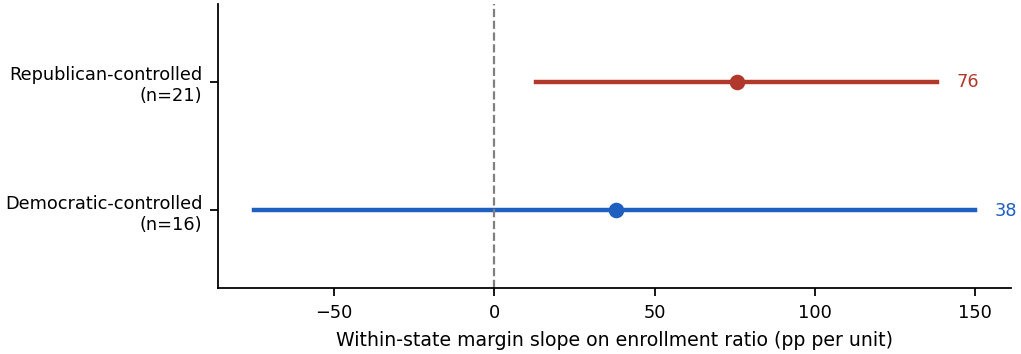
\includegraphics[width=0.60\linewidth]{fig_withinparty.png}
\caption{Within-party margin slope on the enrollment ratio, expansion state-months. Two-way FE coefficient on Democratic seat margin, estimated separately within Republican- and Democratic-controlled chambers; bars are 95\% CIs. The slope is significant only under Republican control, and the two are not statistically distinguishable.}
\label{fig:withinparty}
\end{SCfigure*}

\begin{SCfigure*}[\sidecaptionrelwidth][htbp]
\centering
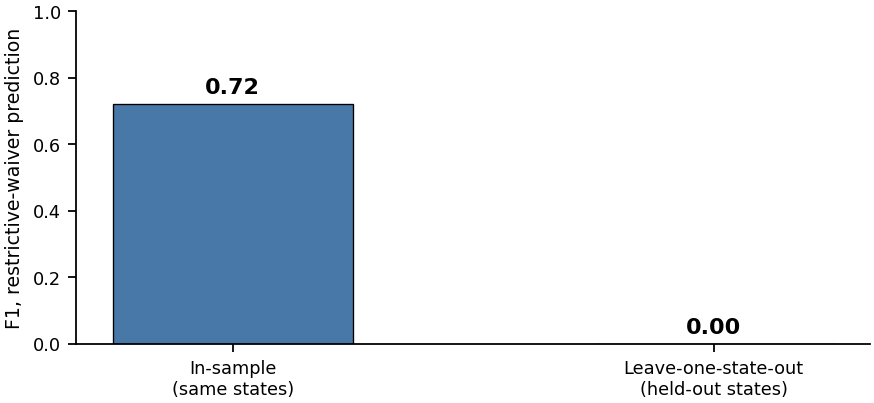
\includegraphics[width=0.60\linewidth]{fig_crossval.png}
\caption{Predicting restriction from seat margin. A depth-3 decision tree fits the training states well (in-sample F1 $=0.72$) but predicts no restriction in held-out states under leave-one-state-out cross-validation (F1 $=0.00$). Majority size does not generalize as a predictor of restriction.}
\label{fig:crossval}
\end{SCfigure*}

\textbf{Placebos.} Consistent with a pattern specific to expansion states, the margin association is statistically zero among non-expansion states (24.7 pp, $p=0.414$) and among pre-expansion months of late expanders (3.8 pp, $p=0.909$). Both placebos are limited---non-expansion states carry little Democratic-margin variation, and the pre-expansion sample is small ($N=456$)---so they are read as directionally consistent rather than decisive (Fig.~\ref{fig:specforest}).

\begin{SCfigure*}[\sidecaptionrelwidth][htbp]
\centering
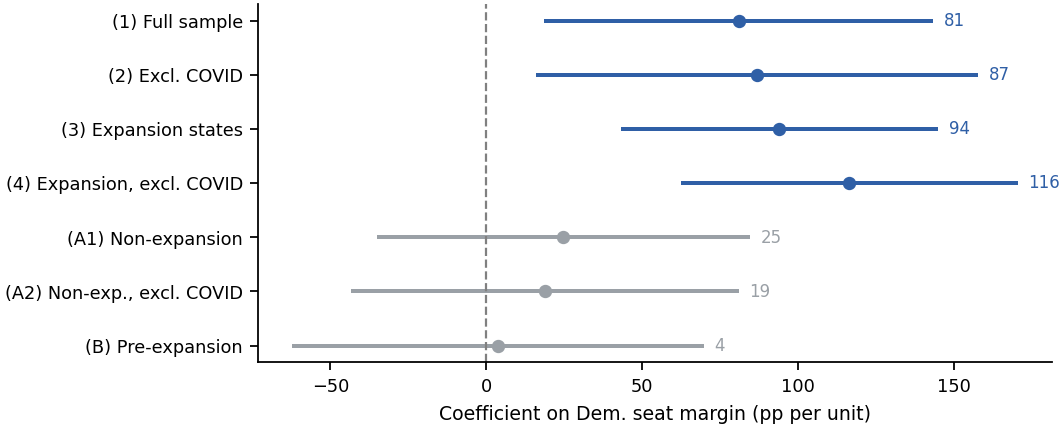
\includegraphics[width=0.60\linewidth]{fig_specforest.png}
\caption{Seat-margin estimates across main specifications (blue) and placebo samples (gray). Two-way FE, state-clustered SEs; bars are 95\% CIs. Main estimates sit away from zero; placebos straddle it but are individually limited.}
\label{fig:specforest}
\end{SCfigure*}

\section*{Discussion}

Across a decade of monthly state data, partisan influence on Medicaid restriction takes the form of a switch rather than a dial. Which party controls the chamber governs whether a state restricts: Democratic-controlled expansion states sit at zero, and restriction appears only under Republican control. But the size of the majority shows no effect the data can detect. The one result that resembles a dial---a positive continuous seat-margin coefficient on enrollment---is identified off the Republican end of the range, is statistically inseparable from direction, fails to predict a single restriction in a held-out state, is discarded by $L_1$ selection in favor of party control, and reverses when one state is removed. The evidence is consistent with a threshold and inconsistent with any detectable continuous gradient: holding the majority is what matters, not its size. A methodological point travels with this. A two-way fixed-effects panel will return a significant ``size'' coefficient that looks like a dial but is a between-state contrast in disguise, because the regressor barely moves within states; cross-validating by state, rather than trusting an in-sample fit, is what tells the two apart.

Two caveats bound the reading. The switch interpretation rests on the discrete separation at control plus the absence of a within-party gradient, not on a sharp estimated cutoff; the data rule out a \emph{detectable} dial, but with one control flip and five composition snapshots the panel is underpowered to resolve the shape just above the threshold. The honest claim is therefore that no dial is detectable here---a failure to reject equality, not a demonstration that the effect is exactly zero---and a setting with more institutional volatility could still surface a faint gradient. And the enrollment outcome mixes a broad numerator with a narrow denominator and absorbs only national shocks through the year effects, which is why restriction, not enrollment, carries the result. The practical implication is direct: for anticipating Medicaid restriction, the legislative variable that matters is which party holds the chamber, not by how much.

\section*{Agentic Analysis}

I used Claude (Anthropic) throughout for code scaffolding, data processing, figure generation, design pressure-testing, and prose editing, in an iterative chat-plus-execution loop; representative transcripts are in the replication repository. The workflow itself was part of the exercise, and the most important lesson concerns scope and skepticism rather than speed.

The project's claim narrowed three times, each time after checking the model's output against the data rather than accepting the cleaner story. An initial framing of ``larger Democratic majorities cover more'' did not survive the observation that the only directly measured mechanism, restrictive waivers, sits entirely on the Republican side. A revised ``Democratic floor'' framing did not survive re-running the within-party split, which showed the Democratic slope to be positive and merely imprecise rather than a true floor. And the surviving ``Republican restriction gradient'' did not survive the leave-one-state-out cross-validation reported here, which reduced it to a single state. In each case the assistant's default was to state the stronger version; each correction came from a numerical check. The assistant also accelerated genuinely useful moves---the state-clustered errors, the placebo samples, and the cross-validation framing of the restriction test---and proposed several extensions (a close-election instrument, an initiative-state design, post-double-selection Lasso) that were correctly relegated to future work rather than allowed to expand a course-scale panel study beyond what its data could support. The central discipline, in the end, was subtraction: fixing one claim the data could carry and declining every elaboration that did not serve it.

\matmethods{All data derive from public sources: KFF State Health Facts, the NCSL Partisan Composition Database, the U.S.\ Census ACS table C17002, and state election returns. Replication code, processed data, and AI transcripts are available at \url{https://github.com/bfloman/QSS20-Final}. The restriction classifier is a depth-3 CART (scikit-learn) evaluated under leave-one-group-out cross-validation with states as groups; the $L_1$ logistic regression uses liblinear with $C=1$.}

\showmatmethods

\begin{thebibliography}{9}
\bibitem{rocco2020} P Rocco, AC Keller, AS Kelly, State politics and the uneven fate of Medicaid expansion. \emph{Health Aff.} 39, 494--501 (2020).
\bibitem{tsebelis2002} G Tsebelis, \emph{Veto Players: How Political Institutions Work} (Princeton Univ.\ Press, 2002).
\bibitem{jarlenski2020} M Jarlenski, et al., Medicaid and state politics beyond COVID. \emph{J. Gen. Intern. Med.} 35, 3401--3404 (2020).
\bibitem{stimson1995} JA Stimson, MB MacKuen, RS Erikson, Dynamic representation. \emph{Am. Polit. Sci. Rev.} 89, 543--565 (1995).
\bibitem{gilenspage2014} M Gilens, BI Page, Testing theories of American politics. \emph{Perspect. Polit.} 12, 564--581 (2014).
\bibitem{berry1998} WD Berry, EJ Ringquist, RC Fording, RL Hanson, Measuring citizen and government ideology in the American states. \emph{Am. J. Polit. Sci.} 42, 327--348 (1998).
\end{thebibliography}

\end{document}
